\documentclass[11pt]{beamer}
\usepackage[utf8]{inputenc}
\usepackage{graphicx, epsfig}
\usepackage{amsmath,mathrsfs,amsfonts,amssymb}
%\usepackage{subfig}
\usepackage{floatflt}
\usepackage{epic,ecltree}
\usepackage{mathtext}
\usepackage{fancybox}
\usepackage{fancyhdr}
\usepackage{multirow}
\usepackage{enumerate}
\usepackage{epstopdf}
\usepackage{multicol}
\usepackage{algorithm}
\usepackage[noend]{algorithmic}
\usepackage{tikz}
\usepackage{blindtext}
\usetheme{default}%{default}%{Singapore}%{Warsaw}%{Warsaw}%{Darmstadt}
\usecolortheme{default}
\setbeamerfont{title}{size=\Huge}
\setbeamertemplate{footline}[page number]{}


\makeatletter
\newcommand\HUGE{\@setfontsize\Huge{35}{40}}
\makeatother    

\setbeamerfont{title}{size=\HUGE}
\beamertemplatenavigationsymbolsempty

% latin bold lower
\newcommand{\ba}{\mathbf{a}} 
\newcommand{\bc}{\mathbf{c}} 
\newcommand{\be}{\mathbf{e}} 
\newcommand{\bh}{\mathbf{h}} 
\newcommand{\bp}{\mathbf{p}} 
\newcommand{\bt}{\mathbf{t}} 
\newcommand{\bs}{\mathbf{s}} 
\newcommand{\bu}{\mathbf{u}} 
\newcommand{\bv}{\mathbf{v}} 
\newcommand{\bw}{\mathbf{w}} 
\newcommand{\bx}{\mathbf{x}} 
\newcommand{\by}{\mathbf{y}} 
\newcommand{\bz}{\mathbf{z}} 

% latin bold upper
\newcommand{\bA}{\mathbf{A}} 
\newcommand{\bB}{\mathbf{B}} 
\newcommand{\bC}{\mathbf{C}} 
\newcommand{\bI}{\mathbf{I}} 
\newcommand{\bL}{\mathbf{L}} 
\newcommand{\bM}{\mathbf{M}} 
\newcommand{\bQ}{\mathbf{Q}} 
\newcommand{\bT}{\mathbf{T}} 
\newcommand{\bU}{\mathbf{U}} 
\newcommand{\bV}{\mathbf{V}} 
\newcommand{\bW}{\mathbf{W}} 
\newcommand{\bX}{\mathbf{X}} 
\newcommand{\bY}{\mathbf{Y}} 
\newcommand{\bZ}{\mathbf{Z}} 

% latin cal upper
\newcommand{\cG}{\mathcal{G}} 
\newcommand{\cL}{\mathcal{L}} 
\newcommand{\cN}{\mathcal{N}} 
\newcommand{\cS}{\mathcal{S}} 
\newcommand{\cT}{\mathcal{T}} 
\newcommand{\cW}{\mathcal{W}} 
\newcommand{\cX}{\mathcal{X}} 
\newcommand{\cZ}{\mathcal{Z}} 

% latin bb upper
\newcommand{\bbE}{\mathbb{E}} 
\newcommand{\bbI}{\mathbb{I}} 
\newcommand{\bbP}{\mathbb{P}} 
\newcommand{\bbR}{\mathbb{R}} 

% greek bold lower
\newcommand{\bepsilon}{\boldsymbol{\epsilon}} 
\newcommand{\btheta}{\boldsymbol{\theta}} 
\newcommand{\blambda}{\boldsymbol{\lambda}} 
\newcommand{\bpi}{\boldsymbol{\pi}} 
\newcommand{\bmu}{\boldsymbol{\mu}} 
\newcommand{\bsigma}{\boldsymbol{\sigma}} 
\newcommand{\bphi}{\boldsymbol{\phi}} 

% greek bold upper
\newcommand{\bSigma}{\boldsymbol{\Sigma}} 

\DeclareMathOperator*{\argmin}{arg\,min}
\DeclareMathOperator*{\argmax}{arg\,max}
\newcommand{\createdgmtitle}[1]{\title[\hbox to 56mm{Mathematical Forecasting Methods \hfill\insertframenumber\,/\,\inserttotalframenumber}]
	{\vspace{1.5\cm} \\ Mathematical Forecasting Methods \\ {\Huge Лекция #1}}
	\author{}
	\institute{
	МФТИ
	} 
	\date{Осень, 2023}
}

\newcommand\myfootnote[1]{%
  \tikz[remember picture,overlay]
  \draw (current page.south west) +(1in + \oddsidemargin,0.5em)
  node[anchor=south west,inner sep=0pt]{\parbox{\textwidth}{%
      \rlap{\rule{10em}{0.4pt}}\raggedright\scriptsize \textit{#1}}};}

\newcommand\myfootnotewithlink[2]{%
  \tikz[remember picture,overlay]
  \draw (current page.south west) +(1in + \oddsidemargin,0.5em)
  node[anchor=south west,inner sep=0pt]{\parbox{\textwidth}{%
      \rlap{\rule{10em}{0.4pt}}\raggedright\scriptsize\href{#1}{\textit{#2}}}};}
\createdgmtitle{11}
\usepackage{tikz}
\usepackage{amsmath}
\usepackage[english,russian]{babel}
\usepackage[labelformat=empty]{caption}

\usepackage{graphicx,animate}
\usepackage{animate}
\usepackage{svg}
\usepackage{subcaption}

\usepackage{ stmaryrd }

\usetikzlibrary{arrows,shapes,positioning,shadows,trees}
\newcommand*{\defeq}{\stackrel{\text{def}}{=}}
\newcommand{\tensor}[1]{\underline{\textbf{#1}}}
\newcommand{\M}[1]{\textbf{#1}}
\newcommand{\norm}[1]{\lVert #1 \rVert }
%--------------------------------------------------------------------------------
\begin{document}
%--------------------------------------------------------------------------------
\begin{frame}[plain]
%\thispagestyle{empty}
\titlepage
\end{frame}
%=======
\begin{frame}{Напоминание}
 

\begin{itemize}
    \item Пусть есть два тензора $\tensor{A} \in \mathbb{R}^{I_1 \times ... \times I_d}$ $\tensor{B} \in \mathbb{R}^{J_1 \times ... \times J_D}$,  тогда назовём  их внешним произведением следующий тензор $\tensor{A} \circ \tensor{B} \in \mathbb{R}^{I_1 \times ... \times I_d \times J_1 \times ... \times J_D}$ с элементами:
$$(\tensor{A} \circ \tensor{B})_{i_1,...,i_d,j_1,...,j_D} = a_{i_1,...,i_d}b_{j_1,...,j_D}.$$

    \item Произведение $n$-ой моды тензора $\tensor{A} \in \mathbb{R}^{I_1 \times \dots \times I_N}$ и матрицы $\M{B} \in \mathbb{R}^{J \times I_n}$ даёт тензор $\tensor{С} \in \mathbb{R}^{I_1 \times \dots \times I_{n-1} \times J \times I_{n+1} \times \dots \times I_N}$ с элементами: $$\tensor{C} = \tensor{A} \times_n^2 \M{B} = \tensor{A} \times_n \M{B}, \quad  c_{i_1, ..., i_{n-1}, j, i_{n+1}, ..., i_N} = \sum_{i_n = 1}^{I_n} a_{i_1, ..., i_n, ..., i_N} b_{j,i_n}$$
    
    \item Мультилинейное произведение (произведение Такера) тензора $\tensor{G}$ и матриц $\M{B}^{(n)}$:

    $$ \tensor{C} = \big[ \tensor{G}; \M{B}^{(1)}, \dots, \M{B}^{(N)} \big] := \tensor{G} \times_1 \M{B}^{(1)} \times_2 \M{B}^{(2)} \times_3 \dots \times_N \M{B}^{(N)} $$
\end{itemize}

\end{frame}
%=======
\begin{frame}{Нормы}

\begin{itemize}
    \item  Норма Фробениуса
    $$\lVert\tensor{A}\rVert_F = \sqrt{\sum_{i_1,...,i_d}|a_{i_1,...,i_d}|^2} = \lVert vec(\tensor{A}) \rVert_2$$
    \item Норма Чебышёва
    $$\lVert\tensor{A}\rVert_С = \max_{i_1,...,i_d}|a_{i_1, \dots, i_d}|$$
    \item Операторная норма 
    $$d=2:
    \norm{A}_2
    = \underset{\norm{\M{v}}_2=1}{sup}\norm{\M{Av}}_2
    = \underset{\M{v} \neq 0}{sup} \frac{\norm{\M{Av}}_2}{\norm{\M{v}}_2} 
    = \underset{\norm{\M{v}}_2=1}{sup}\norm{\llbracket \M{A}; \M{I}, \M{v} \rrbracket}_2
    $$
    $$d>2: \norm{\tensor{A}}_2
    = \underset{\norm{\M{v}^{(1)}}_2=...=\norm{\M{v}^{(d)}}_2=1}{sup}|\llbracket \tensor{A}; \M{v}^{(1)},...,\M{v}^{(d)}\rrbracket|
    $$
    $$
    = \underset{\norm{\M{v}^{(2)}}_2=...=\norm{\M{v}^{(d)}}_2=1}{sup}\norm{\llbracket \tensor{A}; \M{I}, \M{v}^{(2)},...,\M{v}^{(d)}\rrbracket}_2
    $$
\end{itemize}

\end{frame}
%=======
\begin{frame}{Сингулярные числа и векторы}
\begin{itemize}
    \item 
    Неотрицательное число $\sigma \in \mathbb{R}$ называется \textit{сингулярным числом} для матрицы $\M{A} \in \mathbb{R}^{m \times n}$, если существуют векторы $u \in \mathbb{R}^m, \ \norm{u}_2 = 1$ и $v \in \mathbb{R}^n, \ \norm{v}_2 = 1$ такие, что:

\begin{equation}
\label{eq:1}
    \M{Av} = \sigma \M{u}, \quad \M{A}^{\intercal} \M{u} = \sigma \M{v}
\end{equation}

Векторы $\M{u}$ и $\M{v}$ при этом называются, соответственно, \textit{левым и правым сингулярными векторами} $\M{A}$.

\item С помощью операции произведения Такера это представляется так:

$$ \llbracket \M{A}; \M{I}, \M{v} \rrbracket = \sigma \M{u}, \quad  \llbracket \M{A}; \M{u}, \M{I} \rrbracket = \sigma \M{v}$$

\item Отметим, что равенства $\ref{eq:1}$ могут быть получены как необходимые условия стационарной точки в следующей задаче оптимизации:

$$ \max{\M{u}^{\intercal}\M{A}\M{v}}, \quad s.t. \ \norm{\M{u}}_2 = 1, \ \norm{\M{v}}_2 = 1 $$




\end{itemize}
 


%При $d=2$ сингулярные векторы - это критические точки функционала
%$$\frac{\M{w}^{\text{T}}\M{A}\M{v}}{\norm{\M{w}}_2\norm{\M{v}}_2}$$
%Тогда можно записать как 
%$$\llbracket \M{A}; \M{I}, \M{v} \rrbracket = \sigma \M{w}$$
%$$\llbracket \M{A}; \M{w}, \M{I} \rrbracket = \sigma \M{v}$$
%Обобщение на $d>2$ 

\end{frame}
%=======
\begin{frame}{Обобщение сингулярных чисел для тензоров}

\begin{itemize}
    \item  По аналогии с матрицами, можно определить сингулярные вектора тензора $\tensor{A}$ порядка $d$ как стационарные точки следующей задачи:
    $$ \max{\llbracket \tensor{A}; \M{v}^{(1)}, \M{v}^{(2)},...,\M{v}^{(d)}\rrbracket}, \quad s.t. \ \norm{\M{v}^{(1)}}_2 = 1, \dots, \norm{\M{v}^{(d)}}_2 = 1 $$
    \item Аналогично, получим условия на сингулярные числа и сингулярные векторы (единичной длины):
    $$ \llbracket \tensor{A}; \M{v}^{(1)}, \dots, \M{v}^{(k-1)}, \M{I}, \M{v}^{(k+1)}, \dots, \M{v}^{(d)}\rrbracket = \sigma \M{v}^{(k)}, \ k = \overline{1,d}$$
    \item \textbf{Теорема о низкоранговом приближении:} \\
    Наилучшее приближение ранга $1$ для тензора $\tensor{A}$ по норме $\norm{\cdot}_F$ имеет вид $\sigma_1 \M{v}^{(1)} \circ \dots \circ \M{v}^{(d)}$, где $\sigma_1$ -- максимальное сингулярное число тензора, а $\M{v}^{(k)}$ -- соответствующие сингулярные векторы. 
    
\end{itemize}

\end{frame}
%=======
\begin{frame}{Каноническое разложение тензоров (CP-decomposition)}
\vspace{0.1cm}
$\tensor{X} \in \mathbb{R}^{I_1 \times I_2 \times \dots \times I_N}$ - тензор $N$-ого порядка.
\begin{itemize}
    \item Каноническим разложением тензора $\tensor{X}$ называется представление тензора в виде суммы тензоров ранга 1:
    $$ \tensor{X} = \sum_{r=1}^R \M{b}_r^{(1)} \circ \M{b}_r^{(2)} \circ ... \circ \M{b}_r^{(N)} = \sum_{r=1}^R \Bigg( \overset{N}{\underset{n = 1}{\circ}} \M{b}_r^{(n)} \Bigg), \quad \M{b}_r^{(n)} \in \mathbb{R}^{I_n}$$

%  \Leftrightarrow \ x_{i_1, \dots, i_n} = b_{i_1}\dots b_{i_n}

\begin{figure}
    \centering
    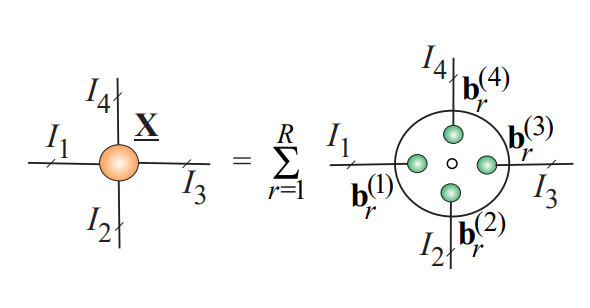
\includegraphics[width=0.6\textwidth]{lecture_11/figs/cp_decomp.png}
\end{figure}

\item \textbf{Определение:} минимальное число слагаемых $R$, необходимое для канонического разложения тензора $\tensor{A}$, называется (каноническим) рангом $\tensor{A}$.
\end{itemize}




\end{frame}
%=======

\begin{frame}{Каноническое разложение через произведение Такера}
\vspace{0.1cm}
$\tensor{X} \in \mathbb{R}^{I_1 \times I_2 \times \dots \times I_N}$ - тензор $N$-ого порядка, \\
индекс $i_n$ пробегает значения $1, \dots, I_n$ для $n = 1, \dots, N$.

\begin{itemize}
    \item Следуя формуле канонического разложения и определению операции внешнего произведения, элемент тензора $\tensor{X}$ представляется в виде:
    $$ x_{i_1, i_2, ..., i_N} = \sum_{r=1}^R b^{(1)}_{r, i_1} b^{(2)}_{r, i_2} \dots b^{(N)}_{r, i_N}$$
    \item Единичным тензором порядка $N$ размера $R$ будем называть тензор c единицами на диагонали:
    $$\tensor{I}_R^N \in \mathbb{R}^{\underbrace{R \times ... \times R}_{N}}, \quad (\tensor{I}_R^N)_{r_1, \dots, r_N} = \begin{cases} 1, & \text{ если } r_1 = r_2 = \dots = r_N \\ 0, & \text{ иначе} \end{cases}.$$
    
    Далее будем опускать индексы $N$ и $R$ и обозначать единичный тензор символом $\tensor{I}$.
\end{itemize}


\end{frame}
%=======

\begin{frame}{Каноническое разложение через произведение Такера}
\begin{itemize}
    \item Сформируем из векторов-элементов канонического разложения $\M{b}_r^{(n)}$ следующие матрицы:

    $$ \M{B}^{(n)} = \Big[ \M{b}_1^{(n)}, \dots, \M{b}_R^{(n)} \Big] \in \mathbb{R}^{I_n \times R}, \quad n = 1, \dots, N$$
    
    \item Наконец, рассмотрим произведение Такера $$\tensor{Y} = \llbracket \tensor{I}; \M{\textbf{B}}^{(1)}, \M{B}^{(2)}, \dots,  \M{B}^{(N)} \rrbracket \in \mathbb{R}^{I_1 \times I_2 \times \dots \times I_N}.$$ Элементы такого тензора имеют следующий вид:
    $$ y_{i_1, i_2, \dots, i_N} = \sum_{r_1=1}^R \sum_{r_2 = 1}^R \dots \sum_{r_N = 1}^R \left(\tensor{I}\right)_{r_1, r_2, \dots, r_N} \M{B}^{(1)}_{i_1, r_1}\M{B}^{(2)}_{i_2, r_2} \dots \M{B}^{(N)}_{i_N, r_N} = $$ 
    $$= \M{B}^{(1)}_{i_1, 1}\M{B}^{(2)}_{i_2, 1} \dots \M{B}^{(N)}_{i_N, 1} +  \dots + \M{B}^{(1)}_{i_1, R}\M{B}^{(2)}_{i_2, R} \dots \M{B}^{(N)}_{i_N, R} = $$
    $$ = \sum_{r=1}^R b^{(1)}_{r, i_1} b^{(2)}_{r, i_2} \dots b^{(N)}_{r, i_N} = x_{i_1, i_2, ..., i_N}$$
\end{itemize}

\end{frame}

%=======

\begin{frame}{Каноническое разложение через произведение Такера}
\begin{itemize}
    \item Сформируем из векторов-элементов канонического разложения $\M{b}_r^{(n)}$ следующие матрицы:

    $$ \M{B}^{(n)} = \Big[ \M{b}_1^{(n)}, \dots, \M{b}_R^{(n)} \Big] \in \mathbb{R}^{I_n \times R}, \quad n = 1, \dots, N$$
    
    \item Наконец, рассмотрим произведение Такера $$\tensor{Y} = \llbracket \tensor{I}; \M{B}^{(1)}, \M{B}^{(2)}, \dots,  \M{B}^{(N)} \rrbracket \in \mathbb{R}^{I_1 \times I_2 \times \dots \times I_N}.$$ Элементы такого тензора имеют следующий вид:
    $$ y_{i_1, i_2, \dots, i_N} = \sum_{r_1=1}^R \sum_{r_2 = 1}^R \dots \sum_{r_N = 1}^R \left(\tensor{I}\right)_{r_1, r_2, \dots, r_N} \M{B}^{(1)}_{i_1, r_1}\M{B}^{(2)}_{i_2, r_2} \dots \M{B}^{(N)}_{i_N, r_N} = $$ 
    $$= \M{B}^{(1)}_{i_1, 1}\M{B}^{(2)}_{i_2, 1} \dots \M{B}^{(N)}_{i_N, 1} +  \dots + \M{B}^{(1)}_{i_1, R}\M{B}^{(2)}_{i_2, R} \dots \M{B}^{(N)}_{i_N, R} = $$
    $$ = \sum_{r=1}^R b^{(1)}_{r, i_1} b^{(2)}_{r, i_2} \dots b^{(N)}_{r, i_N} = x_{i_1, i_2, ..., i_N}$$
\end{itemize}

\end{frame}
%=======

\begin{frame}{Каноническое разложение через произведение Такера}
\begin{itemize}
    \item Два способа представить каноническое разложение:
$$\tensor{X} = \sum_{r=1}^R \M{b}_r^{(1)} \circ \M{b}_r^{(2)} \circ ... \circ \M{b}_r^{(N)} =  \llbracket \tensor{I}; \M{B}^{(1)}, \M{B}^{(2)}, \dots,  \M{B}^{(N)} \rrbracket$$
    \item Иногда на векторы канонического разложения накладывают дополнительное требование $\norm{\M{b}_r^{(n)}}_2 = 1$. Тогда слагаемые умножают на коэффициенты $\lambda_r$, и мы получаем эквивалентную форму:
    $$\tensor{X} = \sum_{r=1}^R \lambda_r \M{b}_r^{(1)} \circ \M{b}_r^{(2)} \circ ... \circ \M{b}_r^{(N)} =  \llbracket \underline{\Lambda} ; \M{B}^{(1)}, \M{B}^{(2)}, \dots,  \M{B}^{(N)} \rrbracket$$
\end{itemize}

\begin{figure}
    \centering
    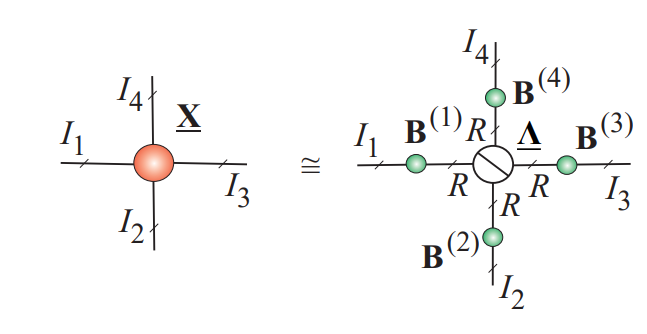
\includegraphics[width=0.55\textwidth]{lecture_11/figs/cp_decomp_2.png}
\end{figure}



\end{frame}






% \begin{frame}{Tensor Train Decomposition}

% $\tensor{X} \in \mathbb{R}^{I_1 \times I_2 \times \dots \times I_N}$ - тензор $N$-ого порядка.

% $$ x_{i_1, i_2, \dots, i_N} = \M{G}_{i_1}^{(1)} \M{G}_{i_2}^{(2)} \dots \M{G}_{i_N}^{(N)}$$ 
% Здесь элемент исходного тензора представлен в виде произведения матриц-сечений тензоров разложения 3-его порядка $\tensor{G}^{(1)}, ..., \tensor{G}^{(N)}$, где $\tensor{G}^{(n)} \in \mathbb{R}^{R_{n-1} \times I_n \times R_n}, \ R_0 = R_N = 1$:
% $$ \M{G}_{i_n}^{(n)} = \tensor{G}^{(n)}\big(:, i_n, : \big), \quad \M{G}_{i_n}^{(n)} \in \mathbb{R}^{R_{n-1} \times R_n}$$

% \end{frame}
%=======
\begin{frame}{Развертка тензора}

$\tensor{X} \in \mathbb{R}^{I_1 \times I_2 \times \dots \times I_N}$ - тензор $N$-ого порядка, \\
индекс $i_n$ пробегает значения $1, \dots, I_n$ для $n = 1, \dots, N$.
\vspace{0.5cm}
\begin{itemize}
    \item Левый мультииндекс (реверсивно-лексикографический):
    $$ \overline{i_1 i_2 \dots i_N} = i_1 + (i_2 - 1)I_1 + (i_3 - 1)I_1 I_2 + \dots + (i_N - 1)I_1 I_2 \dots I_{N-1}$$
    \item Развёрткой $n$-ой моды тензора $\tensor{X}$ называется матрица $$\M{X}_{(n)} \in \mathbb{R}^{I_n \times I_1 I_2 \dots I_{n_1} I_{n+1} \dots I_N},$$  
    $$\Big(\M{X}_{(n)}\Big)_{i_n, \overline{i_1 \dots i_{n-1} i_{n+1} \dots i_N}} = x_{i_1, \dots, i_N}$$

\end{itemize}

\end{frame}
%=======

\begin{frame}{Развертки тензора: иллюстрация}
\begin{figure}
    \centering
    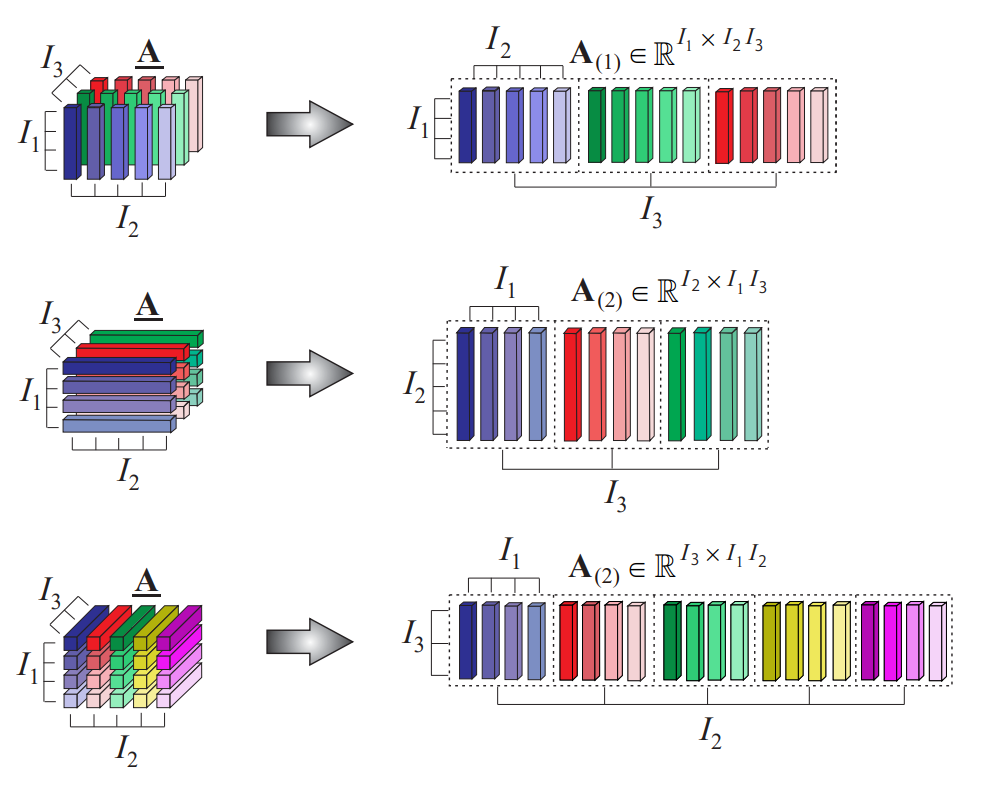
\includegraphics[width=0.9\textwidth]{lecture_11/figs/matricization.png}
\end{figure}
\end{frame}
%=======

\begin{frame}{Развертки тензора: пример}

\begin{minipage}{0.4\textwidth}
\begin{figure}
    \centering
    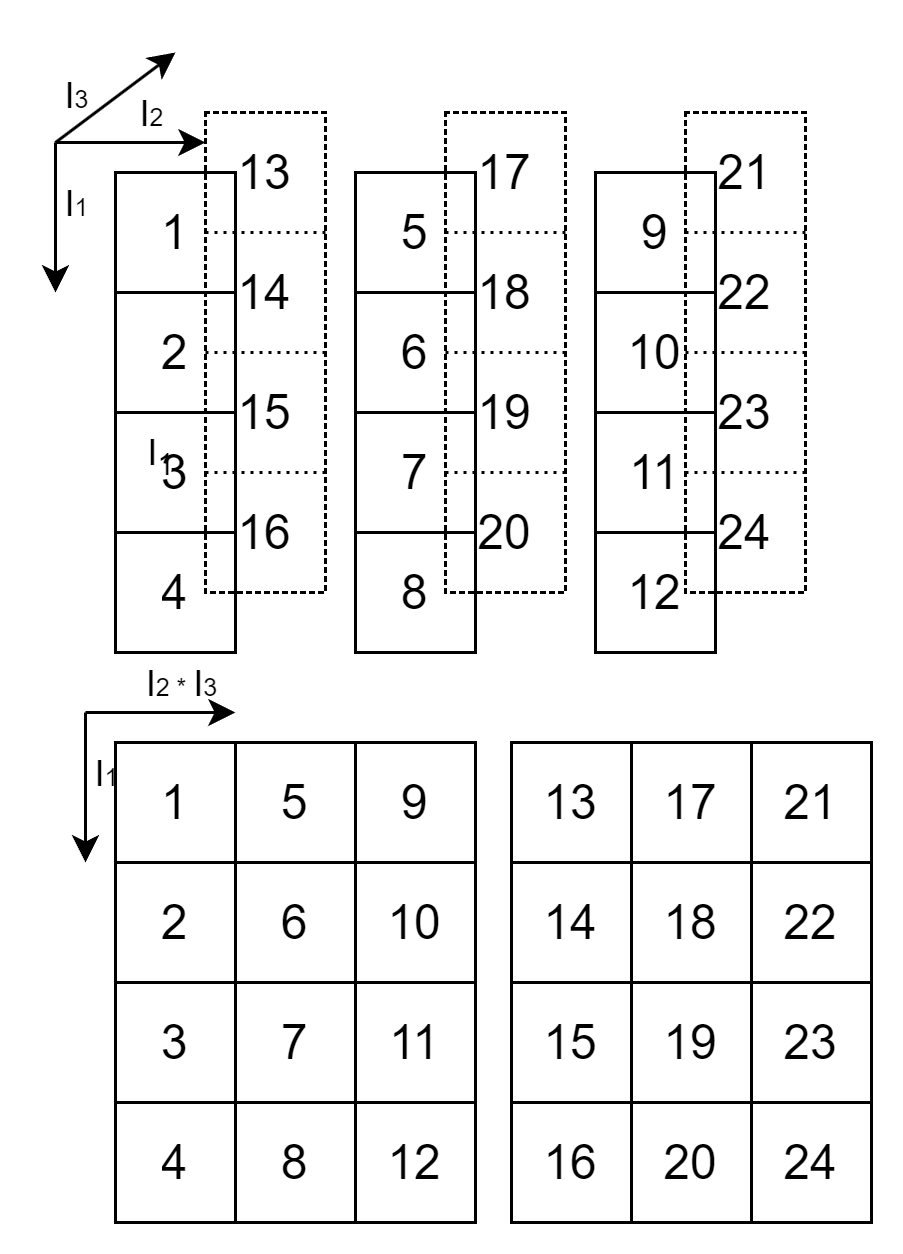
\includegraphics[width=\textwidth]{lecture_11/figs/matricization_example.png}
\end{figure}
\end{minipage}%
\hfill%
\begin{minipage}{0.6\textwidth}%\raggedleft
\begin{itemize}
\item $\tensor{X} \in \mathbb{R}^{4 \times 3 \times 2}$ - тензор $3$-ого порядка
\item Развёрткой $1$-ой моды тензора $\tensor{X}$ называется матрица $$\M{X}_{(1)} \in \mathbb{R}^{4 \times 6} $$
\item Левый мультииндекс
$$ \overline{i_2 i_3} = i_2 + (i_3 - 1)I_2$$
\item Пример $\tensor{X}_{3,1,2} = 15$:
$$\Big(\M{X}_{(1)}\Big)_{3, \overline{1, 2}} = \Big(\M{X}_{(1)}\Big)_{3, 4} = 15$$
\end{itemize}
\end{minipage}


\end{frame}
%=======
\begin{frame}{Кронекерово произведение}


\begin{itemize}
    \item Кронекерово (левое) произведение векторов $\M{a} \in \mathbb{R}^{I_n}$ и $\M{b} \in  \mathbb{R}^{I_m}$ -- это вектор $\M{c}  \in \mathbb{R}^{I_n I_m}$ с элементами:
    $$\M{c} = \M{a} \otimes_L \M{b}, \quad \quad c_{\overline{i_n i_m}} = a_{i_n}b_{i_m}$$

    $$ \M{a} = 
    \begin{bmatrix}
    a_1 \\
    \vdots \\
    a_n 
    \end{bmatrix}, \quad 
    \M{b} = 
    \begin{bmatrix}
    b_1 \\
    \vdots \\
    b_m 
    \end{bmatrix}, \quad
    \M{c} = 
    \begin{bmatrix}
    a_1 b_1 \\
    a_2 b_1 \\
    \vdots \\
    a_n b_1 \\
    a_1 b_2 \\
    a_2 b_2 \\
    \vdots \\
    a_n b_m 
    \end{bmatrix}
    $$
    Порядок следования элементов в векторе $\M{c}$ соответствует левому мультииндексу (реверсивно-лексикографический).
\end{itemize}

\end{frame}


%=======
\begin{frame}{Матричное произведение Хатри-Рао}


\begin{itemize}

    \item Пусть имеются две матрицы c одинаковым количеством столбцов:
    $$ \M{A} = \Big[ \M{a}_1, \dots, \M{a}_R \Big] \in \mathbb{R}^{m \times R}$$
    $$ \M{B} = \Big[ \M{b}_1, \dots, \M{b}_R \Big] \in \mathbb{R}^{n \times R}$$
    \item Произведение Хатри-Рао матриц $\M{A}$ и $\M{B}$ -- это матрица $\M{C}$ со столбцами:

    $$ \M{C} = \M{A} \odot \M{B} = \Big[ \M{a}_1 \otimes_L \M{b}_1, \dots,  \M{a}_R \otimes_L \M{b}_R \Big] \in \mathbb{R}^{mn \times R}$$
    \item С помощью произведения Хатри-Рао удобно выражать развёртки тензоров, представленных в виде произведения Такера. Например, пусть $\tensor{A}$ -- тензор 3-его порядка, и 
    $$ \tensor{A} = \llbracket \tensor{I} ; \M{U}, \M{V},  \M{W} \rrbracket.$$
    Тогда справедливы равенства:
    $$ \M{A}_{(1)} = \M{U} (\M{W} \odot \M{V})^\intercal, \quad \M{A}_{(2)} = \M{V} (\M{W} \odot \M{U})^\intercal, \quad \M{A}_{(3)} = \M{W} (\M{V} \odot \M{U})^\intercal $$
\end{itemize}

\end{frame}
%=======
\begin{frame}{Алгоритмы вычисления CP-разложения: ALS}

\begin{itemize}
    % \item Итеративный процесс оптимизации
    % $$\\
    % \M{B}^{(1)}_{k+1} =  \underset{\M{B}^{(1)}}{argmin} \llbracket \M{B}^{(1)}, \M{B}^{(2)}_{k}, \dots,  \M{B}^{(N)}_{k} \rrbracket \\
    % \M{B}^{(2)}_{k+1} =  \underset{\M{B}^{(2)}}{argmin} \llbracket \M{B}^{(1)}_{k+1}, \M{B}^{(2)}, \dots,  \M{B}^{(N)}_{k} \rrbracket \\
    % \dots \\
    % \M{B}^{(N)}_{k+1} =  \underset{\M{B}^{(N)}}{argmin} \llbracket \M{B}^{(1)}_{k+1}, \M{B}^{(2)}_{k+1}, \dots,  \M{B}^{(N)} \rrbracket$$

    \item Приведём итеративный алгоритм нахождения канонического разложения Alternating Least Squares (ALS) на примере тензора 3-его порядка $\tensor{A}$ (нестрого):
    \vspace{0.5cm}
    \\
    \textbf{Initialize: $\M{U}_1, \M{V}_1, \M{W}_1$} \\
    \textbf{for $k = 1, ..., K$}
    \begin{enumerate}
    \item $\displaystyle U_{k+1} = \argmin_{U}{\norm{\tensor{A} - \llbracket \tensor{I} ; \M{U}, \M{V}_k,  \M{W}_k \rrbracket}_F^2}$
    \item $\displaystyle V_{k+1} = \argmin_{V}{\norm{\tensor{A} - \llbracket \tensor{I} ; \M{U}_{k+1}, \M{V},  \M{W}_k \rrbracket}_F^2}$
    \item $\displaystyle W_{k+1} = \argmin_{W}{\norm{\tensor{A} - \llbracket \tensor{I} ; \M{U}_{k+1}, \M{V}_{k+1},  \M{W} \rrbracket}_F^2}$
    
    \end{enumerate} \\
    \textbf{Output: $\tensor{A} \simeq \llbracket \tensor{I} ; \M{U}_K, \M{V}_K, \M{W}_K \rrbracket$}  \\

\end{itemize}
\end{frame}

%=======

\begin{frame}{Алгоритмы вычисления CP-разложения: ALS}

\begin{itemize}
    \item Рассмотрим подзадачу нахождения оптимальной матрицы $U_{k+1}$. Перейдём под знаком нормы к рассмотрению развёртки тензора вдоль 1-ой моды.
    $$ \displaystyle U_{k+1} = \argmin_{U}{\norm{\tensor{A} - \llbracket \tensor{I} ; \M{U}, \M{V}_k,  \M{W}_k \rrbracket}_F^2} = $$ $$ = \argmin_{U}{\norm{\M{A}_{(1)} -  \M{U} (\M{W}_k \odot \M{V}_k)^\intercal}_F^2 } = $$ $$ = \argmin_{U}{\norm{(\M{W}_k \odot \M{V}_k) \M{U}^\intercal - \M{A}_{(1)}^\intercal}_F^2 }$$
    \item Для полученной задачи выпишем решение в терминах наименьших квадратов:

    $$ U_{k+1}^\intercal = \Big[(\M{W}_k \odot \M{V}_k)^\intercal (\M{W}_k \odot \M{V}_k)\Big]^{-1} (\M{W}_k \odot \M{V}_k)^\intercal \M{A}_{(1)}^\intercal $$

    $$ U_{k+1} = \M{A}_{(1)} (\M{W}_k \odot \M{V}_k) \Big[(\M{W}_k \odot \M{V}_k)^\intercal (\M{W}_k \odot \M{V}_k)\Big]^{-1}$$
\end{itemize}




\end{frame}

%=======

\begin{frame}{Резюме}
\begin{itemize}
    \item Каноническое разложение представляет тензор в виде суммы тензоров ранга 1. Минимальное число слагаемых в таком разложении определяет ранг тензора.
    \item С помощью сингулярных чисел можно определить низкоранговое приближение тензора.
    \item Каноническое разложение можно переписать в терминах произведения Такера.
    \item Операция развёртки тензора позволяет применять к ним аппарат матричной линейной алгебры.
    \item Один из алгоритмов нахождения канонического разложения (ALS) использует представление разложения с помощью произведения Такера, и позволяет итеративно находить матричные компоненты разложения с помощью рассмотрения развёрток тензоров.
\end{itemize}
\end{frame}
\end{document} 